\chapter{Tcl JIT}
\label{tcljit}


\section{A linguagem Tcl}

A linguagem de programação \texttt{Tcl} foi criada em 1989 por John
K. Ousterhout. Ela é interpretada e atualmente sua máquina virtual
trabalha com \textit{bytecodes}. Surgiu como uma linguagem orientada a
comandos para servir a programas interativos, fornecendo tanto uma
interface procedural quanto uma interface textual. A primeira destas é
utilizada por programas que desejam incorporar e estender a
\texttt{Tcl}, a outra permite que usuários programem diretamente com a
linguagem.

Três características básicas diferenciam a \texttt{Tcl} de muitas
outras linguagens: \begin{inparaenum}[(1)]
\item orientada a comandos; \item sintaxe curta; \item tudo é
  \textit{string} UTF--8 (\textit{8-bit Unicode Transformation
   Format})\end{inparaenum}. Um programa qualquer nesta
linguagem pode ser visto como uma sequência de chamadas de funções, onde
cada chamada é descrita pela seguinte EBNF (\textit{Extended
  Backus-Naur Form}): \nomenclature{EBNF}{Extended Backus-Naur Form}
% \cite{ebnfdoc}:
\verb!comando {argumento}!. Cada \verb!comando! invocado pode: já
pertencer a linguagem (\textit{built-in}); ou
ser um comando criado por meio de extensão da linguagem; ou ter
sido criado com a própria \texttt{Tcl}. Os elementos que seguem um comando
são passados como argumentos para o mesmo, deixando o tratamento
semântico destes argumentos por conta do comando. Todo comando retorna uma
\textit{string}, vazia ou não.
\nomenclature{UTF-8}{8-bit Unicode Transformation Format}

Como consequência da primeira característica, \textit{keywords} não
existem na \texttt{Tcl}. Mesmo instruções como
\verb!if! ou \verb!proc! são comandos (esta última é a responsável
pela criação de novos comandos) e podem ser redefinidas, renomeadas ou
removidas pelo usuário.

Por tratar tudo como \textit{string}, os tipos de dados inicialmente
se resumiam a um único tipo. Trabalhos realizados mais tarde
\cite{sah_tc, tcl_bytecode} alteraram esta situação, modificando
a linguagem de forma que possa
haver uma representação interna mais eficiente conforme os valores vão
sendo utilizados. Entretanto, representar tudo como \textit{string} ainda
é característico da \texttt{Tcl} pois essa forma mais eficiente
precisa disponibilizar um meio de recuperar a \textit{string}
representante desta outra forma. É importante ver que certas
operações podem não fazer sentido entre \textit{strings}, como dividir
``abacate'' por ``42''. Sendo assim, indiferente de haver uma
representação interna mais eficiente ou não, os comandos ficam responsáveis
por converter os valores, conforme a necessidade, para outros
tipos para, então, realizar com sucesso ou não sua respectiva operação.


\subsection{Sintaxe e semântica da linguagem}

A sintaxe da \texttt{Tcl} é bastante curta se comparada a outras linguagens
de uso geral. Considerando apenas a semântica da linguagem (e
desconsiderando a semântica de implementação de cada comando), também
tem-se que ela pode ser descrita rapidamente. Para entender como os
comandos são avaliados, discute-se como eles são
formados e entendidos pelo interpretador.

%Comentários são assim considerados somente quando o caractere ``#''
%aparece no lugar de um comando.

Os comandos são separados por ``;'' ou quebra de linha, contanto que
estes elementos não estejam entre aspas duplas ou chaves (``\{'',
``\}''). Separados os comandos, ainda é necessário executá-los. Para
isso, a linguagem realiza duas etapas para cada comando. Na primeira
etapa, a \texttt{Tcl} divide o comando em elementos, cuja definição será
descrita a seguir, e realiza as substituições necessárias que serão
descritas nesta seção. Separados os elementos, a segunda etapa trata de
executar o comando. Para isto, o primeiro elemento é utilizado
para localizar o procedimento associado ao comando e possibilitar sua
execução; os demais elementos são tidos como argumentos para o
procedimento.

Para definir o que são estes elementos mencionados acima, algumas
notações adicionais (palavra simples/composta) à documentação da \texttt{Tcl}
\cite{Tcl.n-manpage} foram estabelecidas aqui. De modo geral, um
elemento pode ser formado por uma palavra simples ou por uma palavra
composta. As palavras simples são
aquelas delimitadas por espaços e não fazem uso de notação adicional.
Considerando o seguinte trecho:
\texttt{puts stderr $\pi$=3},
 que imprime a \textit{string} ``\texttt{$\pi$=3}''
em \verb!stderr!, tem-se três palavras simples. As palavras compostas
são assim chamadas pois podem conter várias palavras simples mas, além
disso, também contém notações especiais. Há três formas de se
construir uma palavra composta. Ao delimitar um conjunto de
palavras simples por aspas duplas, como em: \verb|"olá, mundo!"|,
forma-se uma palavra composta que representa um único parâmetro para
algum comando. Um outro modo envolve trocar as aspas duplas por ``\{''
e ``\}''. Essa troca apresenta efeitos na substituição, que será
tratado adiante. Finalmente, utilizando colchetes também constrõe-se
palavras compostas.

As substituições mencionadas anteriormente são agora descritas. Elas
são divididas em duas: substituição de comandos e substituição de
variáveis. A primeira destas ocorre ao fazer uso da palavra composta
que utiliza colchetes. Para entender o que ocorre na substituição de
comandos, primeiro considere o seguinte trecho de código:
\verb!puts [expr {(1 + sqrt(5))/2}]!, que imprime como resultado
uma \textit{string} cujo conteúdo pode ser interpretado como um número
que aproxima $\varphi$.
O trecho anterior contém dois
elementos: uma palavra simples e outra composta. A palavra composta foi
delimitada por colchetes e, por isso, o interpretador \texttt{Tcl}
entende que esta palavra inicia com um comando e que os demais
elementos são parâmetros para este comando. Sendo assim, a
\texttt{Tcl} avalia esse comando e substitui a palavra composta pelo
resultado obtido. Na palavra composta há ainda outra palavra composta,
mas delimitada por chaves. Nesse caso, não ocorre nenhuma substituição
e o conteúdo entre chaves é repassado para o respectivo comando. No
exemplo anterior, o comando \verb!expr! fica responsável por tratar a
\textit{string} ``\verb!(1 + sqrt(5))/2!''. Caso houvessem outras
palavras compostas delimitadas por colchetes, %chaves,
 a linguagem \texttt{Tcl}
define uma ordem natural de avaliação da esquerda para direita em
sequência.

A substituição de variáveis ocorre nos
casos em que um elemento tem sufixo ``\$", trocando o elemento pelo
valor da variável representada. Há três formatos previstos para esta
substituição: \verb!$var!, \verb!$var(chave)! e
\verb!${var}!. No primeiro caso, \verb!var! descreve o nome de uma
variável escalar. No segundo, \verb!var! é aceito como um \textit{array}
e \verb!chave! é uma \textit{string}, que pode ser formada
por uma palavra composta, que, ao ser avaliada, dá um nome para um
elemento deste \textit{array}. O último caso também se aplica a
variáveis escalares, mas aceita caracteres que desconfigurariam a
situação de palavra simples do primeiro caso. Por exemplo, pode-se
ter o seguinte código: \verb!set {T C L} linguagem!, que, por um
motivo qualquer, define uma variável chamada \verb!T C L! com o valor
\verb!linguagem!. Para imprimir seu conteúdo é necessário, portanto,
utilizar a terceira forma: \verb!puts ${T C L}!.

% * Escape
Uma outra construção sintática existente é a barra invertida. Sua
função é possibilitar a inserção dos caracteres que podem ser
considerados especiais dependendo do contexto (\verb!"!, \verb!$!,
\verb!{!, \verb![!, \verb!\!) e também de outros não imprimíveis.

% * Expansão de argumentos

Com a distribuição da versão 8.5 da \texttt{Tcl}, uma nova
regra precisou ser criada e esse parágrafo dedica-se a ela. A razão
para isto foi a introdução de um recurso denominado expansão de
argumentos. Existe um
conflito parcial com essa regra e o que foi apresentado anteriormente,
então é necessário considerar algumas exceções que ocorrem por meio da
sintaxe para expansão de argumentos. Ao encontrar um elemento com
prefixo ``\verb!{*}!'' com sufixo que não seja caractere em
branco, a expansão de argumentos ocorre. O sufixo é avaliado e
substituído seguindo as regras já mencionadas, em seguida outra
avaliação ocorre. Como resultado pode-se ter diversos elementos. Para
entender esta situação, apresenta-se mais um exemplo:
\begin{verbatim}
set x {puts abacate}
{*}$x
\end{verbatim}
Primeiramente é definido a variável \verb!x! com conteúdo
\verb!puts abacate!. Na linha seguinte é feito uma expansão de argumentos, onde
primeiramente \verb!$x! é avaliada e substituída pelo conteúdo da
variável \verb!x!. Em seguida este mesmo conteúdo é avaliado, causando
a execução do comando \verb!puts! com argumento \verb!abacate!.

% * Comentarios

Finalmente, comentários. A \texttt{Tcl} trabalha com comentários que
se estendem até o final da linha corrente e utiliza o caractere ``\#''
para essa tarefa. Deve-se tomar cuidado ao criar um comentário, o
mesmo só é assim considerado se aparecer no ponto onde o nome de um
comando é esperado. Considere o seguinte trecho de código:
\begin{alltt}
\# Valor aproximado para \(\pi\)
set pi [expr {acos(-1)}]
\end{alltt}
Nesse caso o comentário está correto. Entretanto, mover
o comentário logo em seguida do comando \verb!set!, na mesma linha,
causa um erro. A linguagem entenderia que \verb!#!, \verb!Valor!, e os
demais elementos devem ser passados para o comando \verb!set! que
aceita no máximo três argumentos. Uma outra forma de
causar um comportamento (talvez) não esperado é utilizar ``\#'' no
lugar do nome de um comando dentro de colchetes:
 \verb!puts [# oi]!.
 Apesar do comentário ocorrer num lugar permitido, o colchete que
terminaria o comando foi descartado.

%% Tirei e descrevi tudo a cima.
%\section{Características}
%\label{sec:tcl_caracteristicas}

%\begin{itemize}
%\item exemplos de código destacando as características principais
%\end{itemize}



\section{O Ambiente de Execução}
\label{ambientexec1}

%\begin{itemize}
%\item composição
%\item interação dos componentes
%\item modelo de execução
%\end{itemize}

A \texttt{Tcl} é uma biblioteca em \texttt{C} que inclui um
\textit{parser} para a linguagem \texttt{Tcl}. Para utilizar os
recursos ali existentes, uma aplicação primeiramente obtém, por meio
de uma chamada, um objeto que representa um interpretador. Este objeto
(referência) é a unidade básica de manipulação
da \texttt{Tcl} \cite{ousterhout_89}. A partir dele é possível
acessar a máquina virtual da linguagem (denominada de TVM neste trabalho) e
\nomenclature{TVM}{Tcl Virtual Machine}
proceder para a execução de procedimentos.

A partir da versão 8, a TVM é composta por um compilador que produz
\textit{bytecodes} e trabalha com estes utilizando uma pilha. A
interpretação desta forma de código ocorre essencialmente através da
função \verb!TclExecuteByteCode!, que fica responsável por decodificar
todas as instruções e manter um estado consistente do sistema
simulado.

% A implementação conta
%com um interpretador que
%trabalha juntamente com uma pilha, constituindo a base da sua máquina
%virtual de pilha.

Não há preocupação em definir tipos específicos em momento
algum. Ou a máquina virtual consegue, por meio de funções da
biblioteca, converter um objeto para algum tipo que desejar no momento
que estiver executando uma instrução ou um erro é gerado. Isto
dificulta a criação de compiladores mais eficientes, tendo sido esta
questão discutida nos trabalhos \cite{sah_tc} e
\cite{tcl_bytecode}. Na implementação atual da linguagem há o conceito
de representação dupla para os objetos, sendo uma delas mais eficiente
de se trabalhar. Entretanto, ainda não há uma função, ou algo
semelhante, que dado um objeto qualquer seja retornado seu tipo. Isso
acontece porque dependendo da forma com que se trabalha com um valor,
tipos diferentes podem ser assumidos. Pode-se ter, por exemplo, o
seguinte código:
\begin{verbatim}
set x 4
set $x 2
lindex $x 0
\end{verbatim}
Isto é, primeiramente a variável \verb!x! tem um valor que se parece
com um inteiro mas em seguida este valor é utilizado como um nome para uma
variável e, ainda, depois é tratada como uma lista com um elemento: \verb!4!.

O ambiente é dinâmico, comandos podem ser redefinidos/removidos a qualquer
momento, código pode precisar ser avaliado em tempo de execução ao
fazer uso do comando \verb!eval!, pode-se empregar escopo dinâmico por
meio do comando \verb!uplevel! ou também pode-se simular a passagem
por nomes ao utilizar o \verb!upvar!. Ou seja, a TVM requer cuidados
excessivos para se manter funcionando corretamente. Pode ser
necessário recompilar para \textit{bytecodes} um procedimento
anteriormente compilado, pois o ambiente pode mudar entre chamadas ou
mesmo durante a interpretação de \textit{bytecodes}. De fato, antes de
qualquer execução de um procedimento, é feito uma chamada a função
interna (não exportada pela biblioteca \texttt{Tcl})
\verb!TclProcCompileProc! que determina a necessidade de compilação
(primeira chamada) ou recompilação.

Apenas procedimentos criados através do comando \verb!proc! podem vir
a ser compilados para \textit{bytecodes}. Toda vez que um comando é
criado, a linguagem \texttt{Tcl}
invoca a função \verb!TclCreateProc! para associar a definição de um
procedimento qualquer com uma
estrutura interna \verb!Proc!. Entretanto, somente quando é feito uso do
\verb!proc! é que ocorre a associação entre comando e a função interna
\verb!TclObjInternProc!. Esta
última fica responsável por, indiretamente, chamar a
\verb!TclProcCompileProc! e também a \verb!TclExecuteByteCode! para
efetivamente interpretar o código do procedimento associado.
 Em todos os casos, uma tabela \textit{hash}
de comandos é atualizada quando comandos são criados e permite que,
por meio do nome do comando, a função associada seja acessada pela
máquina virtual para proceder à sua execução.

%Sendo assim, a própria \texttt{Tcl} trabalha num modo misto.

A \texttt{Tcl} trabalha num modo misto, com cada comando do usuário sendo
interpretado por vez mas também permitindo a execução direta de código
\texttt{C}. São utilizados 132 \textit{bytecodes} (na versão 8.5.8)
para converter
código escrito em \texttt{Tcl} para a interpretação pela máquina de
pilha. Cada comando \textit{built-in} da linguagem fornece uma função
para ser chamada durante este processo de compilação, sendo possível
aplicar otimizações em casos bastante específicos. O comando
 \verb!expr!, por
exemplo, é capaz de simplificar o código gerado para expressões
constantes:
 \verb!expr {1 + 2 + 3}! será interpretado como \verb!expr {6}!.
 Para indicar o término de um comando, estas funções
utilizadas para esta compilação emitem a instrução
\verb!INST_DONE!. Ao encontrar este \textit{bytecode}, a máquina
virtual entende que o processo de interpretação daquele comando deve
ser encerrado.

% XXX Falar da contagem de referência como coleta de lixo ?

Em tempo de execução, a máquina virtual faz acesso a dois objetos de
forma mais frequente. Estes objetos são: um \textit{array} de objetos
literais e um \textit{array} de variáveis locais (que também inclui os
argumentos da função). Estes \textit{arrays} são produzidos durante a
geração de \textit{bytecodes} e precisam ser mantidos em um estado
consistente ao longo da execução.
Cada elemento é formado por uma estrutura \verb!Tcl_Obj!,
que é criada para cada objeto no sistema da \texttt{Tcl}. Cuidados
devem ser tomados para não danificar o conteúdo destes
\textit{arrays}, caso contrário uma execução subsequente de um mesmo
comando pode produzir resultados incorretos.

Conhecendo o ambiente ``hostil'' onde o compilador JIT deve ser
instalado, as subseções seguintes descrevem como é feito a instalação do
JIT neste ambiente e quais condições devem ocorrer para que haja
execução de código nativo.

\subsection{Instalação e execução do compilador JIT}
\label{install-exec2}
Para possibilitar a execução do compilador dinâmico em momentos
específicos durante a execução da máquina virtual alvo, algumas
modificações foram realizadas na implementação da
\texttt{Tcl}. Essas modificações efetivamente ``instalam'' o
compilador JIT no sistema original.

Como todo comando está associada a uma estrutura interna \verb!Proc!,
esta estrutura parece ser o local ideal para conter informações
pertinentes a compilação JIT. Isso é devido ao fato de que todos procedimentos
criados, que foram escritos em linguagem \texttt{Tcl}, conterão uma
instância da mesma. Um campo com a estrutura de um
\verb!JIT_Proc! foi adicionado a estrutura \verb!Proc!. A Figura
\ref{jitproc} descreve o conteúdo desta nova estrutura.

\begin{figure}[h]
  \centering
  \begin{tabular}{c}
    \begin{lstlisting}[language=C]
struct JIT_Proc {
  int eligible;
  unsigned int callCount;
  unsigned char *ncode;
  int collectingTypes;
  struct JIT_BCType *bytecodeTypes;
};
    \end{lstlisting}
  \end{tabular}
  \caption{Campos da estrutura JIT\_Proc\label{jitproc}}
\end{figure}

O campo \verb!collectingTypes!, inicializado em \verb!0!, é utilizado para
detectar se já foi alocado memória para o campo \verb!bytecodeTypes!
ou não, sendo atualizado para \verb!1! na primeira execução de uma
função escrita puramente em \texttt{Tcl}. O campo \verb!ncode! é
inicializado em \verb!NULL! e atualizado para um endereço quando for
gerado código de máquina para o procedimento. O campo \verb!callCount!
controla se o procedimento deve ir para compilação dinâmica ou não,
sendo decrementado a cada chamada e estabelecendo que o compilador JIT
deve ser invocado ao atingir
o valor \verb!0!. Atualmente esse campo é inicializado com o valor
\verb!1! (definido por \verb!JIT_REQINVOKE!),
indicando que o procedimento será interpretado uma vez antes
de ser possivelmente compilado e instalado. O primeiro
%de ser possivelmente compilado para código de máquina e instalado em
%seguida. O primeiro
campo, \verb!eligible!, é utilizado para definir se o
procedimento é elegível a compilação dinâmica ou não. A elegibilidade
é definida da seguinte maneira: se alguma execução do procedimento pelo
interpretador retornar um resultado que não seja \verb!TCL_OK!, então
o respectivo procedimento é marcado como não elegível. Isso é feito de
modo a tentar não gerar código que quase certamente terá que
tratar exceções.

Os campos da estrutura \verb!JIT_Proc! requerem
manutenção durante a execução da máquina virtual. Porém, o estado dessa
máquina pode mudar durante execuções subsequentes de um mesmo
procedimento. Se a máquina virtual detectar a necessidade de
recompilação, nesse ponto também aproveita-se para reinicializar os
campos da estrutura \verb!JIT_Proc!
correspondente. A manutenção do campo \verb!bytecodeTypes! é feita por
instrumentação da função \verb!TclExecuteByteCode!,
trechos de código associados a \textit{bytecodes}
relacionados a aritmética e comparação foram incrementados para
realizar a coleta de tipos.


\subsection{Execução do código de máquina}
\label{codeexec}
Uma parte da subseção anterior descreveu em que situação o código de
máquina para um procedimento específico é gerado e instalado. Agora será
apresentado como ocorre a execução do mesmo.

Tomando a estrutura \verb!JIT_Proc! da Figura \ref{jitproc}
%é possível verificar a existência do campo \verb!ncode!, que é
%definido como um ponteiro para \verb!unsigned char!
é possível verificar a existência de informação no campo \verb!ncode!.
A indicação de que um
procedimento \texttt{Tcl} pode ter sua execução realizada por meio de
código de máquina direto ao invés de interpretação é a não nulidade de
\verb!ncode!. Tendo estabelecido um endereço para esse campo é %deve ser
possível requerer que tal endereço seja entendido como um endereço para
uma função. % Se temos um endereço para uma função, devemos conseguir
%invocar tal função passando os parâmetros esperados. A validade dessas
%duas últimas tarefas se deve ao fato de que uma função qualquer é
Isto é válido devido ao fato de uma função qualquer ser
simplesmente uma sequência de \textit{bytes} que foi gerada por algum
compilador para alguma arquitetura. Porém, realizar essa tarefa %essas tarefas
pode
requerer uma certa flexibilidade da linguagem que se deseja
utilizar. No caso da linguagem \texttt{C}, a escolhida para
esse projeto, é permitido realizar um \textit{cast} para %adequado que
resolver esse problema.

Especificamente, o objetivo é tratar o endereço em
\verb!ncode! como um ponteiro para uma função que recebe dois
parâmetros e tem como retorno um valor inteiro, %;
%em seguida invocamos passando os dois parâmetros:
ou seja:
\verb!((int (*)(void *, void *))ncode)(param1, param2)!. A escolha
dessa assinatura é devido àquela existente para a função
\verb!TclExecuteByteCode!. Essa última função é invocada
pela máquina virtual nos casos em que o compilador
JIT não gerou código de máquina para o procedimento. Manter a
compatibilidade, passando os mesmo
parâmetros, proporciona ao código gerado pelo compilador JIT tratar
objetos literais, parâmetros do procedimento \texttt{Tcl}, variáveis
locais e outros detalhes de forma bastante similar ao da
implementação da \texttt{Tcl}.


\section{O Sistema de Compilação}
\label{sistemacompilacao}
% \begin{itemize}
% \item o que compilar
% \item quando compilar
% \item como otimizar
% \end{itemize}

% %\section{O Compilador Dinâmico} % isso não é uma seção mais, juntar
% %                                % com a de cima.
% %\label{sec:tcljit_dinamic}

% \begin{itemize}
% \item estrutura / fases
% \end{itemize}

Satisfazendo as condições base, descritas na subseção
\ref{install-exec2}, o compilador dinâmico pode iniciar seu trabalho.
O sistema desenvolvido trabalha com compilação de procedimentos por
inteiro. A tradução parte dos \textit{bytecodes} existentes,
e somente obtém sucesso se todos eles pertencerem ao subconjunto
aceito pelo compilador
dinâmico atual. Até este momento são aceitos apenas procedimentos folha.

%A coleta de tipos foi criada para tentar guiar o processo de
%compilação. Porém, da forma com que foi feita, ainda não consegue-se
%utilizar os dados coletados de forma eficiente. ... Falar do Psyco que
%faz especialização, etc ...

Diversas simplificações foram feitas para tornar factível a criação
deste novo compilador. Uma delas envolve trabalhar apenas com
instruções que lidam com: manutenção da pilha utilizada pela máquina
virtual, desvio condicional e incondicional, relação entre objetos, aritmética e
lógica. Ainda é assumido que os valores poderão ser tratados como
inteiros limitados ao tamanho da palavra, esta é a restrição mais severa da
implementação atual. Caso um valor realmente não represente um valor
inteiro, então o código gerado tem o cuidado de retornar à
interpretação. Esse desvio faz com que o procedimento seja
interpretado a partir de seu primeiro \textit{bytecode}.
A eliminação de \textit{overhead} de interpretação é decorrente das
simplificações aplicadas e a remoção do custo de decodificação de
instruções é naturalmente obtido pela utilização de código nativo.
%A execução mista entre o interpretador
%\texttt{Tcl} e o compilador JIT possibilita que este último 

%O sistema desenvolvido é fracamente acoplado, sendo necessário ..

Antes de gerar o código nativo, uma outra forma de representação
intermediária, além da existente em \textit{bytecodes}, foi criada.

%Na geração de código ...


%\section{Desenvolvimento}
%\label{desenvolvimento}


\subsection{Representação Intermediária}
\label{intermediate}
%A seguir é apresentado a evolução das escolhas feitas a respeito da
%representação intermediária para o compilador discutido e também o
%estado atual da mesma.

Inicialmente o objetivo era utilizar uma forma de representação
intermediária em árvore. E, em uma etapa mais adiante,
fazer uso de um algoritmo, entre os diversos existentes \cite{noltis,
  ir_tree_parsing, instrselec-dynamic}, para seleção
de instruções baseada em árvores. % Junto com esse fato,
%observa-se que o uso de otimizações durante a geração de código não
%havia sido explicitado no texto anterior.
Porém, a partir da leitura de
textos diversos\cite{dragonbook, muchnick} essa decisão inicial foi repensada de forma a
simplificar o projeto.
%Sendo assim, a etapa de especificação do compilador JIT
%definiu o uso de uma representação intermediária linear de nível
%médio na forma de
%quádruplas.
Com isso, ficou definido o uso de uma representação intermediária
linear de nível médio na forma de quádruplas.
Ainda estava previsto a transformação para a forma SSA \cite{cytron} que
tem sido considerada por diversos compiladores, como LLVM
\cite{llvm1}, GCC \cite{gcc-ssa} e Jalapeño (ou Jikes RVM)
\cite{jalapeno_1}. Tal representação foi deixada para um projeto futuro,
mas vale ressaltar que um dos principais motivos para uso da SSA, de
acordo com \citeonline{cytron}, é a possibilidade de executar
otimizações clássicas de maneira eficiente.
A construção do grafo de fluxo de controle (CFG
-- \textit{Control Flow Graph}) \cite{muchnick} de um trecho de código específico faz
parte dos requisitos para a transformação em SSA, porém ele também é
atualmente utilizado diretamente na geração de código pelo compilador
desse trabalho. Com isso
foi decidido utilizar quádruplas para compor blocos
básicos que representam os nós de um CFG.

A representação em quádruplas é relativamente simples de se construir,
além de apresentar uma característica relevante para a otimização que
realiza movimentação de código: mover uma quádrupla tende a requerer
menor esforço do que rearranjar uma representação em forma de
árvore. Entretanto, conforme discutido em \citeonline{muchnick},
também é possível que a representação em árvore apresente vantagens
em relação à quádruplas, sendo a eliminação de registradores virtuais
temporários e armazenamentos nos mesmos uma delas.

Na versão atual do compilador a estrutura apresentada na Figura
\ref{quad-struct} representa uma quádrupla.

\begin{figure}[h]
  \centering
  \begin{tabular}{c}
    \begin{lstlisting}[language=C]
struct Quadruple {
  Value *dest;
  unsigned char instruction;
  Value *src_a, *src_b;
  struct Quadruple *next;
};
     \end{lstlisting}
   \end{tabular}
  \caption{Estrutura para uma quádrupla\label{quad-struct}}
\end{figure}

O campo \verb!instruction! tem tipo \verb!unsigned char! pois atualmente
representa um dos \textit{bytecodes} da \texttt{Tcl} ou uma das
instruções \verb!JIT_INST_SAVE!, \verb!JIT_INST_MOVE!, %\verb!JIT_INST_CALL!,\\
\verb!JIT_INST_GOTO!, \verb!JIT_INST_JTRUE!, \verb!JIT_INST_JFALSE!,
\verb!JIT_INST_INCR! e \verb!JIT_INST_NOP!,
que podem ser representadas com um
\textit{byte} (todas elas tem um número associado no intervalo [0, 255]). Essas
novas instruções foram criadas para eliminar detalhes da máquina de
pilha ou para deixar mais claro seu significado. No caso da
\verb!JIT_INST_SAVE!, ela apenas substitui o uso do nome da instrução, da
\texttt{Tcl}, \verb!INST_DONE! mas faz a mesma tarefa:
salva um objeto \verb!Tcl_Obj! para representar o resultado da
avaliação do procedimento e também se prepara para retornar um código
(sucesso ou falha). A \verb!JIT_INST_MOVE! é utilizada para agrupar os
\textit{bytecodes} \verb!INST_PUSH1!, \verb!INST_PUSH4!,
\verb!INST_LOAD_SCALAR1!, \verb!INST_LOAD_SCALAR4!,
\verb!INST_STORE_SCALAR1! e \verb!INST_STORE_SCALAR4! que possuem
pouca diferença, na implementação atual, para a geração de código.
As novas instruções de desvio eliminam a
necessidade de distinção entre o uso de 1 ou 4 \textit{bytes} para
indicar o destino do desvio. O comando \verb!incr! da \texttt{Tcl}
aceita um valor inteiro qualquer como incremento, mas, para poder fazer uso
de instruções de máquina mais eficientes, foi criada a instrução
\verb!JIT_INST_INCR! que opera somente com os valores 1 e -1.
A intrução \verb!JIT_INST_NOP! foi adicionada
porque não há nada equivalente nos \textit{bytecodes} da \texttt{Tcl},
e é utilizada em casos específicos na construção da representação
intermediária descritas mais adiante.

O campo \verb!next!, da Figura \ref{quad-struct}, existe para
lidar de forma eficiente com casos de otimização que requerem a
movimentação de código, apesar de otimizações ainda não terem sido
implementadas. Os campos de tipo \verb!Value!,
inicialmente, permitiam assumir valores inteiros, ponteiros para
\verb!Tcl_Obj! ou uma forma de registrador. Na versão atual essa
estrutura contém os campos \verb!flags! e \verb!offset!. O
primeiro é utilizado para indicar onde o valor deverá
ser encontrado em tempo de execução. O segundo indica um deslocamento
para o valor caso o mesmo se encontre em um \textit{array}.

A Figura \ref{struct-bb} dscreve a estrutura utilizada para agrupar as
quádruplas e formas or blocos básicos.

\begin{figure}[h]
  \centering
  \begin{tabular}{c}
    \begin{lstlisting}[language=C]
struct BasicBlock {
  int id;
  int exitcount;
  struct Quadruple *quads, *lastquad;
  int *exitblocks;
};
    \end{lstlisting}
  \end{tabular}
  \caption{Estrutura para um bloco básico\label{struct-bb}}
\end{figure}

Como não há um campo ``\verb!next!'' nessa abstração, \verb!exitcount!
guarda o número de arcos que saem de um bloco de modo a
permitir o controle de sua travessia por meio do campo
\verb!exitblocks!. O ponteiro \verb!lastquad! é
utilizado na construção do CFG, eliminando a necessidade de travessia das
quádruplas presentes em um bloco para identificar se a última
instrução é de desvio ou não. O campo \verb!id! serve, até o momento,
somente para \textit{debugging}. A identificação dos blocos básicos e
construção do CFG não difere daquela apresentada em
\citeonline{muchnick}, porém não é feito, até o momento, o
uso de blocos básicos estendidos.% A visualização dos blocos básicos
%ainda não ocorre de forma didática, sendo possível apenas uma exibição
%em modo texto bastante simples; com algum esforço é possível
%transformar essa saída em uma entrada para algum programa que trata do
%desenho de grafos.
% Em breve
%espera-se gerar código na linguagem \texttt{dot} ou fazer uso do
%aplicativo xfig para facilitar essa tarefa. Ainda assim é possivel
%analisar o que é gerado e, para isso, tomamos o código exemplo seguinte:
 %Para visualizar os blocos básicos, e tornar
%mais fácil a verificação, foi criada uma função que escreve na
%linguagem \texttt{dot} o conteúdo contido nessas estruturas. Dado um
%código como:

%Para exemplificar um CFG construído, consideremos o procedimento
Para exemplificar a construção de um CFG é considerado o procedimento
descrito na Figura \ref{fig:gray}.

% ???
\begin{figure}[h]
  \centering
  \begin{tabular}{c}
    \begin{lstlisting}%[language=Tcl]

proc palindromo {n} {
  set num $n
  set inv 0
  while {$num} {
    set digito [expr {$num % 10}]
    set inv [expr {$inv * 10 + $digito}]
    set num [expr {$num / 10}]
  }
  expr {$n == $inv}
}
    \end{lstlisting}
  \end{tabular}
  \caption{Procedimento que determina se um número $n$ é considerado palíndromo\label{fig:gray}}
\end{figure}

%Feita uma pequena modificaação na implementação é possível definir
%\verb!JIT_REQINVOKE! em 0 e, antes da primeira execução interpretada do
%código, conseguimos exibir o CFG. Ao executar ``\verb!grayb 2!''
%teremos que a função \verb!JIT_Compile! (nome segue o padrão de
%nomenclatura do código fonte da \texttt{Tcl} para funções públicas)
%será chamada pela função
%\verb!TclObjInterpProcCore!, essa última foi modificada conforme
%descrito na subseção \ref{install-exec}.
Após a execução do procedimento
\verb!JIT_Compile! tem-se como resultado o grafo de fluxo de
controle. A construção do mesmo ocorre em duas etapas, o resultado da
primeira é apresentado na Figura \ref{bbs}.
%Essa última é invocada pela própria
%\texttt{Tcl} e fica responsável por chamar a função que realiza a
%interpretação de \textit{bytecodes}, a
%\verb!TclExecuteByteCode!. Pretende-se realizar a coleta de tipos
%durate a execução dessa última função mencionada, alterando-a de
%acordo com as necessidades do compilador JIT. Enfim, ao término
%da função \verb!JIT_Compile! o grafo de fluxo de controle exibido a
%seguir é obtido.

\begin{figure}[ht!]
  \centering
  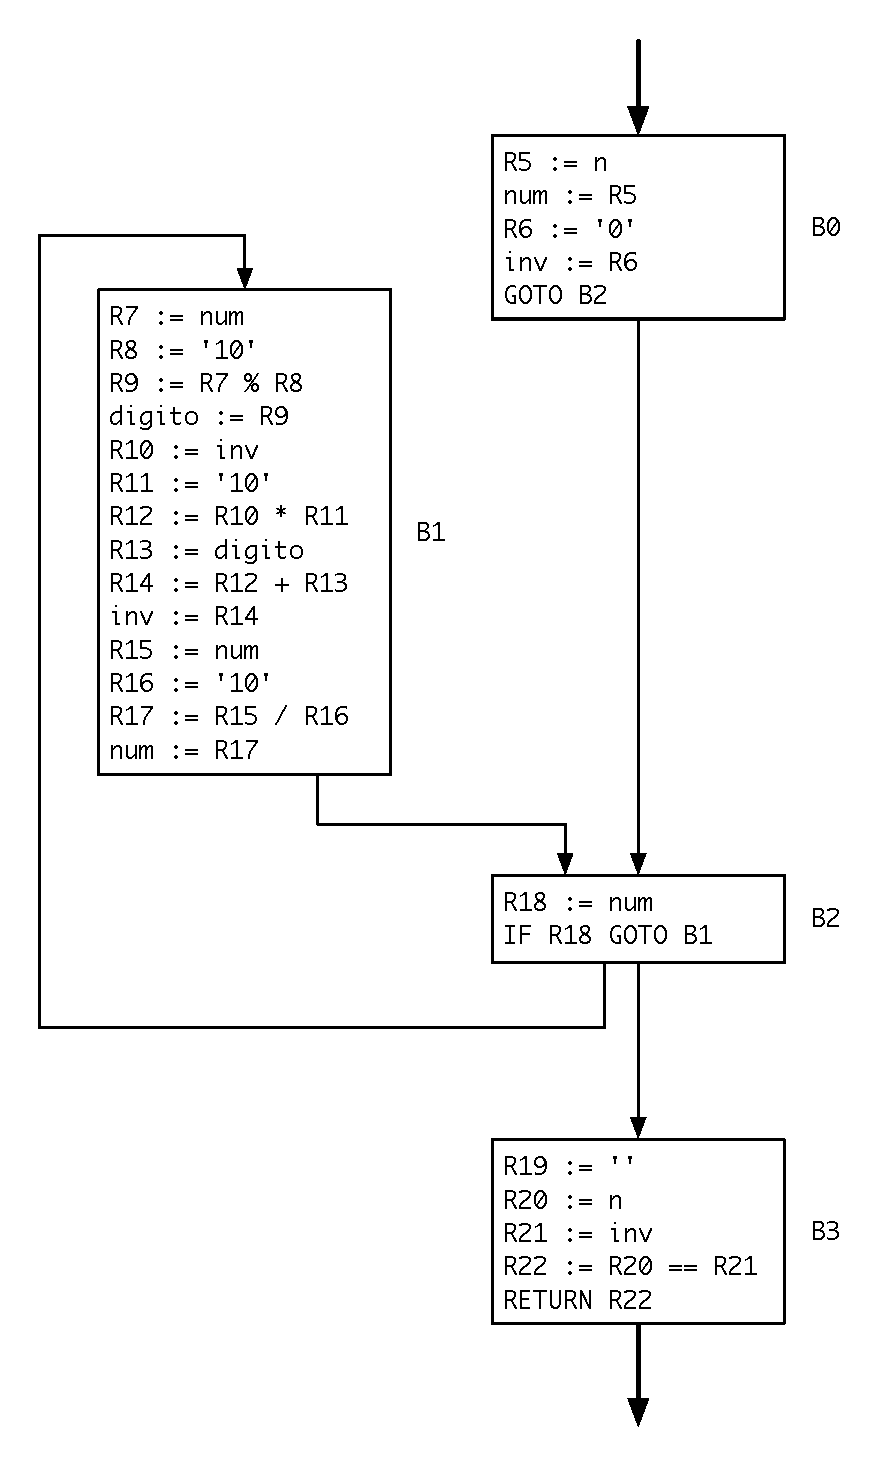
\includegraphics[scale=0.68]{figs/palindromo_bbs1}
  \caption{Blocos básicos e grafo de fluxo de controle construídos,
    etapa 1 \label{bbs}}
\end{figure}

Para se chegar a esta representação foi feita uma conversão de
máquina virtual baseada em pilha para algo semelhante a
uma máquina de infinitos registradores. Uma pilha temporária é
utilizada para simplificar essa transição, sendo acessada e atualizada
durante a construção de diversas instruções. Também são pré-alocados
registradores virtuais para as variáveis locais. A implementação da
\texttt{Tcl} disponibiliza uma lista dinâmica com todas as
variáveis locais, incluindo também os parâmetros formais da função,
sendo necessário apenas atribuir índices a elas. Os registradores que se
enquadram nessa lista tiveram seus nomes alterados para simplificar a
visualização. O registrador \verb!R1! foi renomeado para \verb!n! na
Figura \ref{bbs}, \verb!R2! para \verb!num!, \verb!R3! para \verb!inv!
e \verb!R4! para \verb!digito!.

Diversas instruções de atribuição recebem um
valor que se parece com número, como \verb!'0'! ou \verb!'10'!, mas
que estão sendo representados como \textit{strings}. Na realidade esses valores
são ponteiros para uma estrutura \verb!Tcl_Obj!, podendo assumir
qualquer tipo interno presente na linguagem. No exemplo anterior estes
dados realmente serão convertidos para inteiros. % A
%\textit{string} \verb!'puts'! armazenada no registrador 4 servirá como chave em uma tabela \textit{hash} que possui como valor a
%respectiva função (ou não, gerando um erro).
Todos esses ponteiros
estarão armazenados em um \textit{array} quando a função for executada,
sendo necessário definir os campos \verb!flags! e \verb!offset! da
estrutura \verb!Value! correspondente.
%O número entre parênteses na instrução \verb!CALL!
%indica que haverá 1 parâmetro na chamada e, no caso, este será o
%conteúdo de \verb!R9!.
%A única instrução no bloco de saída B3 indica o
%valor de retorno de função -- uma \textit{string} vazia.

Após construir os blocos básicos iniciais (Figura \ref{bbs}), uma
segunda etapa de construção é realizada. Nesta fase, as quádruplas que
tiverem operandos \verb!Tcl_Obj! serão
movidas para um bloco básico ``especial'' e, ainda, aquelas que
operarem sobre um parâmetro serão também copiadas para esse novo bloco
e a quádrupla original será ajustada. Essa etapa foi desenvolvida
baseando-se na observação de como os
\textit{bytecodes} são interpretados. Na Figura \ref{bbs}, todos
os \verb!Tcl_Obj! presentes são oriundos do \textit{array} de objetos
literais (Seção \ref{ambientexec1}). Carregar estes elementos têm um
custo tanto em quantidade de \textit{bytes} produzidos quanto no
desempenho do código nativo. No bloco básico 1, pode-se ver que há 3
movimentações de objetos literais (representado por '10'). Nos blocos 0 e 3
há dois acessos envolvendo o parâmetro formal. É mais simples
realizar movimentação entre registradores do que acessar o '10'
por meio de um \textit{array} que precisará ser percorrido a cada
iteração do laço. De modo semelhante, é mais eficiente primeiramente
carregar o valor recebido em um parâmetro para um registrador e operar
sobre ele do que buscar
seu valor atual no \textit{array} de variáveis locais. Com essas
transformações, a representação atualizada é exibida na Figura \ref{bbs2}.

\begin{figure}[ht!]
  \centering
  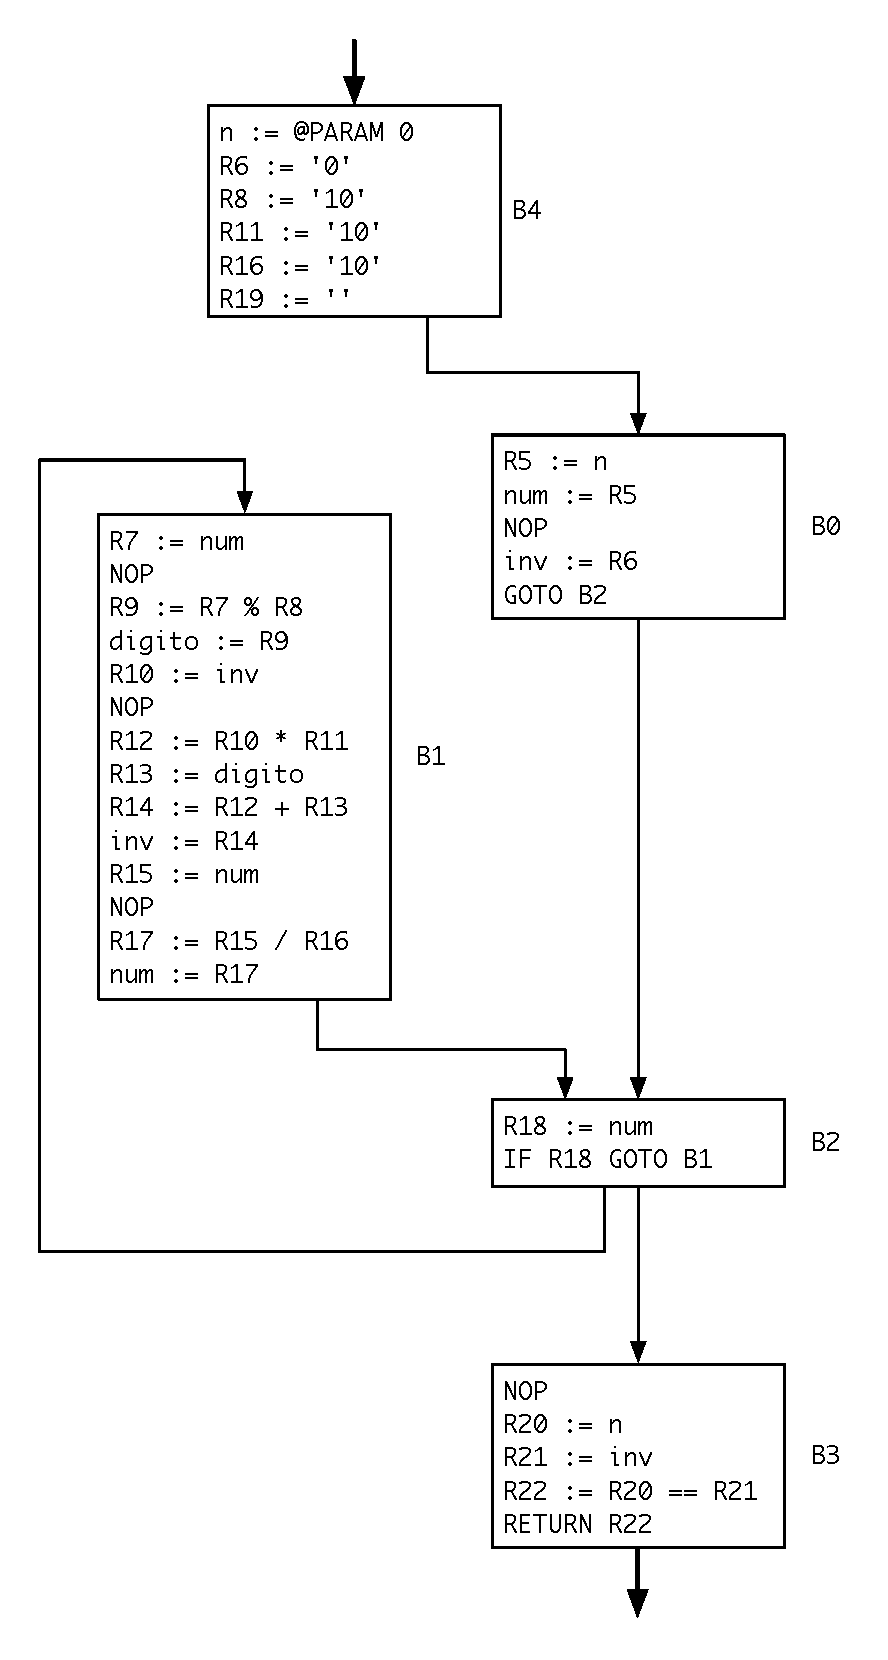
\includegraphics[scale=0.68]{figs/palindromo_bbs2}
  \caption{Blocos básicos e grafo de fluxo de controle final\label{bbs2}}
\end{figure}

Na Figura \ref{bbs2}, o bloco básico chamado de ``especial'' tornou-se
o bloco inicial. A primeira quádrupla ali contida indica que o
parâmetro na posição 0 do \textit{array} de variáveis locais deve ser
carregada para um registrador onde $n$ vive. As instruções \verb!NOP!
ficam a cargo do gerador de código decidir entre emitir código para
cada uma ou não. Essa segunda etapa traz ainda outro benefício. Se um
objeto \verb!Tcl_Obj! não puder ser transformado para um número
inteiro, então logo no primeiro bloco essa situação é detectada. Isso
permite que a volta ao interpretador ocorra de forma mais rápida.
% Com essa representação final surge outra oportunidade
%de otimização, ... olha só o R6, R8, R11 e R16 tudo com o mesmo
%objeto.. poderia utilizar só um.

O código da Figura \ref{fig:gray} utiliza 107 \textit{bytecodes}, aqui
(Figura \ref{bbs2}) representado com 32 quádruplas.
%Haviam 55 \textit{bytecodes} (não exibidos aqui) sendo utilizados para
%representar o código da figura \ref{fig:gray}, e agora 18 quádruplas
%são empregadas com o mesmo resultado. Nessa quantidade numérica
%superior destaca-se o uso de 9 bytes para representar a instrução
%\verb!INST_START_CMD! da \texttt{Tcl}, destinando 1 byte para o código
%da instrução em si, 4 bytes para indicar a posição relativa do início
%do próximo comando e
%4 bytes para contar a quantidade de comandos que fazem parte desse que
%está iniciando de modo a possibilitar ao  interpretador respeitar
%limites impostos para certos recursos por meio de
%APIs específicas. Porém,
Apesar das quádruplas estarem em número inferior,
%levando em conta o total de bytes contidos em cada quádrupla (de
%acordo com as estruturas acima) tem-se que
o consumo de memória é bastante superior (mas temporário), pois após
a geração de código as quádruplas não precisam mais estar em memória.
%Ao mesmo tempo é possível observar que muitas delas são passíveis a
Além disto, algumas são passíveis a
eliminação, ficando a cargo desta eliminação etapas de otimização.
 % otimizações em etapas futuras.

%Um último esclarecimento a respeito da figura \ref{bbs} precisa ser feito.
Os \textit{bytecodes} de desvio emitidos pela \texttt{Tcl} utilizam
operandos que descrevem posições relativas (negativas ou positivas) à
posição atual, porém, na
representação utilizada há somente desvios absolutos para blocos
básicos. Para essa tarefa cada
\textit{bytecode} é mapeado para cada bloco básico antes da construção do
conteúdo dos blocos, assumindo que não existirão mais quádruplas do que
\textit{bytecodes}.

\subsubsection{Mapeamento de alguns \textit{bytecodes} para quádruplas}

A seguir é realizada uma breve análise de como alguns
\textit{bytecodes} são convertidos para quádruplas. O exemplo da
Figura \ref{fig:limiar} é tomado como base para a discussão.

% XXX ?? Erro com tabular e language=Tcl
\begin{figure}[h]
  \centering
  \begin{tabular}{c}
    \begin{lstlisting}%[language=Tcl]

proc limiar-bipolar {x} {
  if {$x >= 0} {
    return 1
  } else {
    return -1
  }
}
    \end{lstlisting}
  \end{tabular}
  \caption{Procedimento exemplo para análise \textit{bytecodes}
    $\rightarrow$ quádruplas\label{fig:limiar}}
\label{xx$xx}
\end{figure}

%Ao executar tal código o interpretador gera uma exceção. Porém, antes de
%exibir a descrição do problema, a função \verb!JIT_Compile! é
%invocada (assumindo que \verb!JIT_REQINVOKE! ainda está definida em \verb!0!).
A Tabela \ref{tabela1} apresenta, lado a lado, os \textit{bytecodes}
produzidos pela \texttt{Tcl} e o código intermediário gerado pelo
compilador JIT para o procedimento
da Figura \ref{fig:limiar}. Para simplificar a visualização dos
\textit{bytecodes}, fez-se uso de \textit{labels} que não existem no
código produzido pela \texttt{Tcl}.

\begin{table}[h]
  \centering
  \caption{Saída produzida para procedimento da Figura \ref{fig:limiar} \label{tabela1}}
  \begin{tabular}{| p{4cm} | p{4cm} |}
    \hline
    \bf{Bytecode} & \bf{Registradores} \\
\begin{verbatim}
LOAD_SCALAR x
PUSH '0'
GE
JUMP_FALSE label1

START_CMD
PUSH '1'
DONE
JUMP label2

label1: START_CMD
PUSH '-1'
DONE

label2: DONE
\end{verbatim} &
\begin{verbatim}
R2 := x
R3 := '0'
R4 := R2 >= R3
IF NOT R4 GOTO B2


R5 := '1'
RETURN R5
GOTO B3

B2:
R6 := '-1'
RETURN R6

B3:
\end{verbatim} \\
    \hline
  \end{tabular}
\end{table}

%Os registradores R2 e R3 contém endereços de memória
%estruturados como \verb!Tcl_Obj!. Por esse motivo, não
%há um endereço previsto para a variável \verb!x! e, portanto, esse
%código certamente geraria um erro se fosse compilado para código de
%máquina.%  Corrigindo,
% alterando para imprimir \verb!$::x!, a seguinte sequência de bytecodes
% e de registradores é produzida:

% \begin{table}[h]
%   \centering
%   \caption{Saída produzida para procedimento corrigido da figura 5}
%   \begin{tabular}{| p{4cm} | p{4cm} |}
%     \hline
%     \bf{Bytecode} & \bf{Registradores} \\
% \begin{verbatim}
% PUSH 'puts'
% PUTS '::x'
% LOAD_SCALAR_STK
% INVOKESTK 2
% DONE
% \end{verbatim} &
% \begin{verbatim}
% R1 := 'puts'
% R2 := '::x'
% ...
% CALL R1 (1) R2
% \end{verbatim} \\
%     \hline
%   \end{tabular}
% \end{table}

%%% NEXT_INST_V(1, 1, 1)

%O processo de mapear um determinado \textit{bytecode} para quádruplas
%é simples. Este processo será descrito detalhando as informações
%contidas na Tabela \ref{tabela1}.

%Continuando ainda no exemplo da figura \ref{fig:global1}, detalhamos
%como o mapeamento de uma coluna para outra foi realizado no restante
%dessa seção. Começando pela
%A instrução \verb!DONE! %vemos que nada equivalente aparece na coluna
%a direita.  por exceções e tão pouco
%por código de retorno anormal -- embora tais tarefas sejam realizadas em
%diversos pontos da máquina virtual..

O lado direito da Tabela \ref{tabela1} representa o resultado da etapa
1 da construção de CFG, o resultado final da etapa 2 não auxiliaria no
propósito desaa discussão.

A instrução \verb!START_CMD!
não possui uma quádrupla equivalente. Isso é resultado da
atual simplificação feita. Diferentemente
da máquina virtual, o código nativo não verifica se o procedimento
sendo executado foi alterado e simplesmente assume que isso não
ocorrerá.

A instrução \verb!PUSH! é mapeada utilizando uma pilha temporária e
um \textit{array} de objetos literais. Um operando que segue a
instrução \verb!PUSH! é tomado como o índice do \textit{array}.
O registrador criado neste ponto,
\verb!R3! no exemplo, é então empilhado. A instrução \verb!LOAD_SCALAR!
é mapeada de forma similar, mas ela se baseia em obter o
endereço da variável escalar de uma lista de variáveis locais
criada pelo compilador da \texttt{Tcl} para o procedimento
corrente. Neste ponto os registradores R2 e R3 estão na pilha e
a instrução \verb!GE! deve ser convertida. Típico de uma máquina de
pilha, esta instrução não requer que ela seja seguido de operandos
pois os mesmos equivalem aos dois últimos empilhados. Da mesma forma,
a pilha artificial criada é utilizada para simular esse comportamento.
O resultado da comparação é empilhado, mas a representação utilizada
pelo compilador dinâmico também requer que tal resultado seja
armazenado em um novo registrador.

Para converter a instrução de desvio \verb!JUMP_FALSE!, a pilha
utilizada é consultada para descobrir qual registrador contém um valor
que determina a realização do desvio ou não. O destino é calculado
utilizando o mapeamento mencionado no final da Seção \ref{intermediate}.

% Seguida de um
%operando, chamado de \verb!objc!, indicando a quantidade total de
%argumentos (incluindo o nome da função) os elementos
%$0 \dots objc - 2$ da pilha a partir do topo são os parâmetros para
%a função na posição $objc - 1$ a partir do topo. Na representação
%utilizada não é considerado o nome da função como um parâmetro, por isso
%entre parênteses está o número 1 ao invés do 2.
A instrução \verb!DONE! é utilizada para indicar um ponto de
retorno, sua conversão para o modelo de registradores consiste
simplesmente em retornar o último objeto empilhado. Nota-se que a
última instrução
não teve código produzido, isso é devido a uma heurística aplicada de
que uma sequencia de instruções \verb!DONE! equivale a uma única.

\subsection{Geração de Código de Máquina}
\label{codegen}
Após descrever como a representação intermediária é construída e
o funcionamento do sistema para
executar o código gerado, o próximo passo é descrever como tal
código de máquina é gerado considerando o uso de uma arquitetura CISC
(\textit{Complex Instruction Set Computer}) e, em específico, a
IA-32 \cite{intel_basicarch}.
\nomenclature{CISC}{Complex Instruction Set Computer}

%Logo após a criação do CFG, a função \verb!JIT_CodeGen! é invocada e o
%seu resultado é um ponteiro para \verb!unsigned char! que em seguida é
%passado para um campo \verb!ncode! de um procedimento específico. A
%função \verb!JIT_CodeGen! faz todo o trabalho que cabe a
%esta seção.

\subsubsection{Reservando e controlando espaço para os bytes}
%A primeira questão a ser tratada é onde colocar os bytes que serão
Um ponto importante é decidir onde armazenar os bytes que serão
gerados. De acordo com a Seção \ref{codeexec}, uma função é apenas uma
sequência de bytes que pode ser executada. De forma direta é possível
pensar em armazenar os bytes em um região de memória alocada por
uma função como \verb!malloc!. Porém, simplesmente fazer isso não garante
que o sistema operacional permitirá a execução desta sequência de bytes.

Com a introdução do bit NX (\textit{No-eXecute}) pela AMD e depois
pela Intel (que renomeou para \textit{eXecute-Disable}), o hardware
passou a prevenir a execução de código em páginas destinadas a
dados \cite{intel_prog} e, dessa forma, eliminar
parcialmente ataques relacionados a \textit{buffer
  overflow}\footnote{O artigo ``Code Injection Attacks on
  Harvard-Architecture Devices'' de Aurélien Francillon e Claude
  Castelluccia publicado na ACM CCS 2008 menciona trabalhos que
  contornam a proteção por bit NX além de outras proteções que
  tem sido desenvolvidas.}.
Por essa razão uma região de
memória alocada por meio do \verb!malloc! não poderá ter seu conteúdo
executado em sistemas que fazem uso desse recurso. Uma forma de
contornar esse problema é utilizar a função \verb!mprotect!,
definindo a região com proteção de leitura e execução após escrever os dados
desejados. Entretanto, essa função requer que o tamanho da região
alocada seja um múltiplo do tamanho de página -- denominado de
\textit{page-aligned}. Para contornar este outro problema é possível
utilizar a função
\verb!memalign! ou \verb!valloc!, de acordo com a disponibilidade. Porém,
o mais adequado é definir o tamanho da região como um múltiplo do
tamanho de página, eliminando a necessidade de alinhamento e reduzindo
questões de portabilidade. % A quantidade de bytes que define o tamanho
%de uma página pode ser obtido com a função
%\verb!getpagesize!.
A estrutura exibida na Figura \ref{mcode-struct}
juntamente com as funções% \verb!pagesize!, \verb!newpage! e
%\verb!pagenowrite!
 exibidas no Apêndice \ref{apendiceA}
tratam dos problemas mencionados %de forma similar a descrita
 e também
de questões de portabilidade entre os sistemais operacionais Windows e UNIX.

\begin{figure}[h]
  \centering
  \begin{tabular}{c}
    \begin{lstlisting}[language=C]
struct MCode {
  unsigned char *mcode, *codeEnd;
  int limit, used;
};
    \end{lstlisting}
  \end{tabular}
  \caption{Estrutura para controlar uso de memória do código gerado\label{mcode-struct}}
\end{figure}

Os campos \verb!limit! e \verb!used! determinam o tamanho total
alocado e o espaço usado até o momento, respectivamente. Atingindo o
valor limite, uma nova página precisa ser alocada e o campo
\verb!limit! tem seu valor dobrado. Os campos \verb!mcode! e
\verb!codeEnd! apontam para o início do código de máquina e o
ponto atual na região de memória, respectivamente. O endereço contido em
\verb!mcode! é o que será instalado no campo
\verb!ncode! da estrutura \verb!JIT_Proc! de um procedimento
específico caso a geração de código tenha sucesso.


\subsubsection{Início e término da geração}
\label{begin-end-codegen}

Antes de gerar código específico para um CFG, é gerado um prólogo
genérico que pode ser visto na 
Figura \ref{prologo-epilogo}. Após a geração de código para o CFG é
gerado um epílogo que também é
apresentado na Figura \ref{prologo-epilogo}. O código gerado pode
lidar com registros de ativação de tamanho variado, por isso é
definido um ponto base para acessar
% A divisão da pilha em
%partes (\textit{frames}) origina o conceito de \textit{stack frame}
%que é manuseado pelo código do prólogo. Cada \textit{stack frame} pode
%variar de tamanho, e por isso definimos um ponto base para acessar
parâmetros ou variáveis locais de forma que seja respeitada as
condições da ABI \cite{systemv-abi}. Essa base, ou ponto de
referência, fica definida como 
o endereço contido no registrador \verb!ebp! após a execução do
prólogo. É possível encontrar definições de prólogo que incluam código
para salvar os registradores \verb!ebx!, \verb!edi!, \verb!esi!
e \verb!esp! uma vez que, de acordo com a ABI seguida, esses
registradores (além do \verb!ebp! que já é salvo) precisam ser
preservados entre chamadas. Na
implementação atual, código para salvar qualquer um desses
registradores precisa ser gerado conforme necessário. O epílogo possui
código antônimo daquele contido no prólogo, efetivamente desfazendo o
registro de ativação construído e retornando para o endereço contido
na topo da pilha corrente.

\begin{figure}[ht!]
  \centering
  \begin{lstlisting}[language=C, numbers=left]
#define PROLOGUE(code, stsize) {  \
  PUSH_REG(code, EBP); \
  MOV_REG_REG(code, ESP, EBP) \
  if (stsize > 0) { \
    if (4 * stsize > 127) { SUB_IMM32_REG(code, 4 * stsize, ESP); } \
    else { SUB_IMM8_REG(code, 4 * stsize, ESP); } \
  } \
}

#define EPILOGUE(code, stsize) { \
  if (stsize > 0) { \
    if (4 * stsize > 127) { ADD_IMM32_REG(code, 4 * stsize, ESP); } \
    else { ADD_IMM8_REG(code, 4 * stsize, ESP); } \
  } \
  LEAVE(code); RETN(code) \
}

#define PUSH_REG(code, reg) *code++ = 0x50 + reg
#define MOV_REG_REG(code, src, dest) \
    *code++ = 0x89;                  \
    *code++ = MODRM(0x3, src, dest)
#define LEAVE(code) *code++ = 0xC9
#define RETN(code) *code++ = 0xC3

#define ADD_IMM8_REG(code, imm, reg) \
    *code++ = 0x83; \
    *code++ = MODRM(0x3, 0, reg); \
    *code++ = imm
#define ADD_IMM32_REG(code, imm, reg) \
    *code++ = 0x81; \
    *code++ = MODRM(0x3, 0, reg); \
    IMM32(code, imm)
#define SUB_IMM8_REG(code, imm, reg) \
    *code++ = 0x83; \
    *code++ = MODRM(0x3, 0x5, reg); \
    *code++ = imm
#define SUB_IMM32_REG(code, imm, reg) \
    *code++ = 0x81; \
    *code++ = MODRM(0x3, 0x5, reg); \
    IMM32(code, imm)

#define MODRM(mod, reg, rm) (mod << 6) + (reg << 3) + rm

#define IMM32(code, v) \
    *code++ = v; *code++ = v >> 8; \
    *code++ = v >> 16; *code++ = v >> 24
  \end{lstlisting}
  \caption{Código completo para epílogo e prólogo em x86\label{prologo-epilogo}}
\end{figure}

Para os códigos exibidos adiante assume-se que \verb!code! seja um
ponteiro da forma do \verb!codeEnd!
da estrutura \verb!MCode! (Figura \ref{mcode-struct}) e disponha de
uma região de memória suficiente para a execução correta dessas macros.

Na Figura \ref{prologo-epilogo}, o código entre as linhas 1 e 16, é
semelhante com código em \texttt{Assembly} \cite{assembly1} de sintaxe
AT\&T \cite{sintaxeatt}. A partir da linha 18 é semelhante, porém
simplificado, a um montador para x86. Para entender o significado das
linhas 18, 20, 21 e 42, a Tabela \ref{mov-push-1} apresenta uma descrição
sucinta das instruções \verb!MOV! e \verb!PUSH!.
% com formato
%similar àquelas encontradas nos  manuais da Intel
%\cite{intel_aam}\cite{intel_naz} mas
%adaptada para sintaxe AT\&T e reduzida para as necessidades da situação.

\begin{table}[ht!]
  \caption{Uma variação das instruções MOV e PUSH\label{mov-push-1}}
  \centering
  \begin{tabular}{l l l l c}
    \toprule
    Opcode  & Instrução     & Operando 1    & Operando 2    &  Modo 64-Bits \\
    \midrule
    0x89 /r & \verb!MOV r32, r/m32!& ModRM:reg (r) & ModRM:r/m (w) &  Válido       \\
    0x50+rd & \verb!PUSH r32!      & reg (r)       &               &  N.C.         \\
    \bottomrule
  \end{tabular}
\end{table}

A coluna ``\textit{Opcode}'' apresenta
os códigos hexadecimais das variações de \verb!MOV! e \verb!PUSH!
utilizadas e também as informações ``/r'' e ``+rd''. A primeira
indica que a instrução faz uso de um byte chamado de ModR/M, que é
dividido em três partes: mod (2 bits),
reg/opcode (3 bits) e r/m (3 bits), da direita para esquerda seguindo
a ordem \textit{little-endian}. O formato final do byte é formado conforme
a linha 13 da Figura \ref{prologo-epilogo}.
A parte ``reg/opcode'' determina ou um
número de registrador ou mais três bits de informação de acordo com
a especificação do \textit{opcode} (que não é utilizado aqui). O campo
``r/m'' ou específica um registrador como um operando ou pode ser
combinado com o ``mod'' para codificar um modo de endereçamento. Para
mais detalhes sobre o byte ModR/M recomenda-se a consulta ao manual da
\citeonline[capítulo 2]{intel_aam}. Além disto,
a informação ``+rd'' indica que um código entre 0
e 7, simbolizando um registrador de 32 bits, deve ser somado ao valor
em hexadecimal. A segunda coluna indica que os operandos são
registradores de 32 bits (\verb!r32!) ou que pode-se buscar algum
conteúdo no endereço de memória calculado (\verb!r/m32!). No
caso dessa variação do \verb!MOV! o objetivo é mover dados de um
registrador para outro. A última coluna da tabela indica se o
\textit{opcode} apresentado pode ser utilizado no modo 64-bits ou não;
no caso do \verb!PUSH! está indicado que a sintaxe da instrução
não é codificável no modo 64-bits. Ou seja, essa última coluna
indica quais das instruções atualmente codificadas pelo
compilador teriam que ser no mínimo ajustadas para gerar código para
uma arquitetura x64.

A informação contida entre parênteses ``r'' ou ``w'', indica
que o conteúdo do operando será lido
(\textit{\textbf{r}ead}) ou atualizado
(\textit{\textbf{w}ritten}) pelo processador.
 Para a instrução \verb!MOV! é possível utilizar 32 combinações de
endereçamento, devido ao uso do byte ModR/M. Entretanto, o interesse é
apenas na especificação de registradores. De acordo com a
Tabela 2.2 do manual em \citeonline[seção 2.1.5]{intel_aam}
é necessário estabelecer o campo ``mod'' do byte ModR/M em 3 para
essa situação e, assim, juntamente com os números dos registradores fonte e
destino é possível completar esse byte adicional. Dessa forma, a
linha 9 do código da Figura \ref{prologo-epilogo} está resolvida.


\subsubsection{Percorrendo Blocos e Gerando Código}

O gerador de código percorre os blocos básicos do CFG por meio de uma
busca em profundidade e emite código para as instruções contidas em
cada bloco. Durante o percurso do CFG, cada quádrupla
do bloco básico corrente é acessada e um
\textit{switch} de instruções define qual cláusula corresponde a
instrução contida na quádrupla.

Devido a granularidade alta, imposta pela representação intermediária
atual, mesmo instruções simples requerem uma quantidade
relativamente alta de \textit{bytes} para codificá-las. Para realizar
uma discussão detalhada, faz-se uso de uma única instrução de
multiplicação.

O exemplo da Figura \ref{myinc} gera 2 blocos básicos com um total de 5
quádruplas, o processo de tradução de \textit{bytecodes} é exibido na
Tabela \ref{tabela-processo}.

% XXX ?? Erro estranho se deixar language=Tcl
\begin{figure}[ht!]
  \centering
  \begin{tabular}{c}
    \begin{lstlisting}%[language=Tcl]

proc twice {x} {
  expr {$x * $x}
}
    \end{lstlisting}
  \end{tabular}
  \caption{Código exemplo para análise da geração de código \label{myinc}}
\end{figure}

\begin{table}[ht!]
  \centering
  \caption{Processo de conversão do código da Figura \ref{myinc} \label{tabela-processo}}
  \begin{tabular}{| p{2.8cm} | p{3.3cm} | p{3.4cm} | p{5cm} |}
    \hline
    \bf{Bytecode} & \bf{CFG, etapa 1} & \bf{CFG, etapa 2} & \bf{Instruções}\\
\begin{verbatim}
LOAD_SCALAR x
LOAD_SCALAR x
MULT
DONE
\end{verbatim} &
\begin{verbatim}
BB0:
  R2 := x
  R3 := x
  R4 := R2 * R3
  RETURN R4
\end{verbatim} &
\begin{verbatim}
BB1:
  R1 := @PARAM 0
BB0:
  R2 := R1
  R3 := R1
  R4 := R2 * R3
  RETURN R4
\end{verbatim} &
\begin{verbatim}
LOAD_SCALAR src, dest
JIT_INST_MOVE src, dest
JIT_INST_MOVE src, dest
INST_MULT s1, s2, dest
JIT_INST_SAVE src
\end{verbatim} \\
    \hline
  \end{tabular}
\end{table}

A última coluna da Tabela \ref{tabela-processo} identifica as
instruções representantes de cada quádrupla.
Os nomes das instruções que não
começam com \verb!JIT_! foram reaproveitados da \texttt{Tcl}.
Outra informação contida
diz respeito a quantidade de \textit{bytes} a serem reservados na
pilha, definindo o parâmetro \verb!stsize! para o código do prólogo e
epílogo da Figura \ref{prologo-epilogo}. Por tratar-se de um compilador não
otimizador, também não é aplicado uma fase de alocação de
registradores. Por isso, cada registrador virtual é mapeado para um
endereço na pilha e seus endereços são derivados a partir do seu
número exibido nas figuras anteriores.

Ao encontrar uma instrução \verb!LOAD_SCALAR!, o gerador de código
sabe que precisará armazenar uma variável local em uma posição da
pilha. A Seção \ref{codeexec} descreveu a assinatura
da função criada pelo compilador JIT, sem detalhar os tipos dos argumentos.
Para manter a compatibilidade com as estruturas internas do ambiente de
execução, o primeiro parâmetro é uma estrutura
interna \verb!Interp! que será utilizada para acessar a
variável local. A partir desta informação, os \textit{bytes} gerados que
imediatamente seguem o prológo gerado são referentes a movimentação do
primeiro parâmetro para um registrador. O código na Figura
\ref{copy-param} realiza essa primeira função de acordo com a ABI escolhida.


\begin{figure}[ht!]
  \centering
  \begin{tabular}{c}
    \begin{lstlisting}[language=C]
#define COPY_PARAM_REG(code, paramn, reg) \
  MOV_DISP8DREG_REG(code, 8 + 4 * paramn, EBP, reg)

#define MOV_DISP8DREG_REG(code, disp, src, dest) \
  *code++ = 0x8B;                              \
  *code++ = MODRM(0x1, dest, src);             \
  *code++ = disp
    \end{lstlisting}
  \end{tabular}
  \caption{Cópia de parâmetro para registrador seguindo ABI escolhida\label{copy-param}}
\end{figure}

Assumindo um uso da forma:
\verb!COPY_PARAM_REG(code, 0, EAX)!, será possível encontrar em tempo de 
execução o endereço de uma estrutura \verb!Interp! no registrador 
\verb!eax!. Vale ressaltar o uso de outra variação
da instrução
\verb!MOV! aqui (em complemento àquela da Tabela \ref{mov-push-1}),
 que é traduzida para \texttt{Assembly} como:
\verb!movl disp(%src), %dest!. Nesse ponto é possível atravessar a
estrutura \verb!Interp! até
alcançar o \textit{array} que contém todas as variáveis locais, utilizando
trecho de código apresentado na Figura \ref{goto-varstruct}.

\begin{figure}[ht!]
  \centering
  \begin{tabular}{c}
    \begin{lstlisting}[language=C]
long int offset;
offset = offsetof(Interp, varFramePtr);
MOV_DISP8DREG_REG(code, offset, EAX, EAX);
offset = offsetof(CallFrame, compiledLocals);
MOV_DISP8DREG_REG(code, offset, EAX, EAX);
    \end{lstlisting}
  \end{tabular}
  \caption{Percorrendo Interp até variáveis locais\label{goto-varstruct}}
\end{figure}


A estrutura \verb!Interp! possui o campo \verb!varFramePtr! que
aponta para um \verb!CallFrame!. 
A estrutura \verb!CallFrame!, por sua vez, possui um
\verb!array! de tipo \verb!Var!, chamado de \verb!compiledLocals!,
que armazena as variáveis locais. Portanto, a Figura
\ref{goto-varstruct} gera código equivalente a:
\verb!interp->varFramePtr->compiledLocals!, assumindo
que \verb!interp! aponte para o parâmetro de tipo
\verb!Interp!. Após isso, é utilizado o campo
\verb!offset! da estrutura \verb!Value! de \verb!src_a!, deslocando em
\verb!compiledLocals! até o ponto desejado e tornando possível acessar
o \verb!Tcl_Obj! que representa a variável local procurada (código
apresentado na Figura \ref{goto-localvar}, que é a continuação do
código da Figura \ref{goto-varstruct}). A
variável é um parâmetro para a função
escrita em \texttt{Tcl}. Além disso, é o primeiro argumento e, por
essa razão, o deslocamento será 0 no \verb!array! \verb!compiledLocals!.

\begin{figure}[h]
  \centering
  \begin{tabular}{c}
    \begin{lstlisting}[language=C]
#define ADD_IMM8_REG(code, imm, reg) \
  *code++ = 0x83;                  \
  *code++ = MODRM(0x3, 0, reg);    \
  *code++ = imm


if (src_a->offset) {
  ADD_IMM8_REG(code, sizeof(Var) * src_a->offset, EAX);
}
offset = offsetof(Var, value.objPtr);
MOV_DISP8DREG_REG(code, offset, EAX, EAX);
    \end{lstlisting}
  \end{tabular}
  \caption{Acessando variável local\label{goto-localvar}}
\end{figure}

Após acessar o objeto desejado, é possível obter o valor inteiro
contido no mesmo (se houver). Objetos \verb!Tcl_Obj! contém uma
estrutura responsável por armazenar o valor inteiro (assim como os
demais tipos existentes), mas não há
garantias de que o mesmo contenha um valor válido mesmo se o objeto
``parecer'' ser um número. Por essa razão, é necessário fazer uso da
função \verb!Tcl_GetLongFromObj! que verifica se a representação em
\textit{bytes} do objeto pode ser convertida para um inteiro e, então,
atualiza a sua representação interna mais eficiente com o valor
obtido. Sendo assim, e seguindo o modelo simplificado mencionado no
ínicio da Seção \ref{sistemacompilacao}, a conclusão da codificação da
instrução \verb!LOAD_SCALAR! requer uma chamada a
\verb!Tcl_GetLongFromObj!, verificação de erro e armazenamento do
valor obtido. A Figura \ref{fimloadscalar} apresenta o código
utilizado neste momento.

%  Entretanto, o endereço desse objeto será
% reutilizado antes do código de máquina terminar e, portanto, é
% necessário salvá-lo
% em outro registrador (se possível). O código na
% Figura \ref{inc-tclobj} avança até o ponto em que o valor contido no
% objeto é incrementado, simplificações são feitas de modo que é
% assumido que o objeto já construiu uma representação de tipo inteiro.

\begin{figure}[h]
  \centering
  \begin{tabular}{c}
    \begin{lstlisting}[language=C]
AND_IMM8_REG(code, -16, ESP); /* Alinhamento */
PUSH_REG(code, EBX);          /* calle-save  */

/* End. mem. para armazenar valor inteiro. */
LEA_DISP8DREG_REG(code, staddr, EBP, EDX);

PUSH_REG(code, EDX);          /* End. armaz. valor */
PUSH_REG(code, EAX);          /* (Tcl_Obj *) */
PUSH_DISP8DREG(code, 8, EBP); /* (Interp *) */

MOV_IMM32_REG(code, (ptrdiff_t)Tcl_GetLongFromObj, EBX);
CALL_ABSOLUTE_REG(code, EBX);

ADD_IMM8_REG(code, 12, ESP);
POP_REG(code, EBX);

/* Verificar por cod. retorno. */
CMP_IMM8_REG(code, 0, EAX);
JUMP_NOTEQ(code, ``LINTERP'');
    \end{lstlisting}
  \end{tabular}
  \caption{Conclusão da instrução LOAD\_SCALAR \label{fimloadscalar}}
\end{figure}

Na Figura \ref{fimloadscalar}, o variável \verb!staddr!
refere-se a um endereço na pilha calculado por meio campo
\verb!offset! do registrador virtual. O alinhamento da pilha à 16
\textit{bytes} é feito por causa da ABI do sistema operacional Mac OS
X \cite{macosx-abi}, que exige este alinhamento para chamadas de
funções mesmo na arquitetura IA-32. Um outro ponto a considerar neste
código, é a verificação de código de erro. Esse rótulo \verb!LINTERP!
(última linha da Figura \ref{fimloadscalar})
aparece logo abaixo do epílogo criado inicialmente (Subseção
\ref{begin-end-codegen}), agindo como um
outro epílogo mas que define o conteúdo do registrador \verb!eax! como
sendo \verb!JIT_RESULT_INTERPRET!. Quando essa posição do código é
atingida, significa que a suposição de que os valores seriam inteiros
falhou e o código deve ser interpretado pela TVM.

As duas instruções \verb!JIT_INST_MOVE! que seguem são mais simples de
serem codificadas. Cada uma realiza apenas a movimentação do conteúdo de
um endereço de pilha para outro endereço de pilha, fazendo uso de duas
instruções \verb!MOV!.

A instrução \verb!INST_MULT! carrega o conteúdo de dois endereços de
pilha para registradores, aplica a instrução \verb!IMUL! e
armazena o resultado na posição de pilha descrita pelo registrador
virtual de destino.

Nesse momento o resultado de $x^2$ foi calculado, mas existe a
necessidade de retornar esse valor num formato aceito pelo restante do
ambiente. Essa é a tarefa da instrução \verb!JIT_INST_SAVE!.
De acordo com o funcionamento da \texttt{Tcl}, é
necessário definir o objeto resultado da função \verb!twice! para o
interpretador em que a função executa. Efetivamente não é feito
uso de interpretador aqui, entretanto é necessário armazenar
um objeto \verb!Tcl_Obj! em \verb!interp->objResultPtr! pois possívelmente será acessado
por outros comandos \texttt{Tcl} por meio da função \verb!Tcl_GetObjResult!.
Para preencher esse requerimento é feito uso da função
\verb!Tcl_NewLongObj! e \verb!Tcl_SetObjResult!. A primeira é
utilizada para criar um \verb!Tcl_Obj! com o valor resultante de
$x^2$, a segunda é responsável por armazenar o objeto criado pela
primeira no lugar adequado.
Somente depois dessas tarefas é possível
retornar o código \verb!TCL_OK! (\verb!0!) para indicar sucesso.
O código contido nas Figuras \ref{myinc-last-macros} e \ref{myinc-last}
realiza essas tarefas finais.

% Nesse momento a variável local já foi incrementada mas ainda
% existe a necessidade de realizar algumas tarefas antes de retornar. De
% acordo com o
% funcionamento da \texttt{Tcl}, é
% necessário definir o objeto resultado da função \verb!myinc! para o
% interpretador em que a função executa. Efetivamente não é feito
% uso de interpretador aqui, entretanto é necessário armazenar uma cópia desse
% \verb!Tcl_Obj! em \verb!interp->objResultPtr! pois possívelmente será acessado
% por outros comandos \texttt{Tcl} por meio da função \verb!Tcl_GetObjResult!.
% Para preencher esse requerimento é feito uso da função \verb!Tcl_SetObjResult!.
% Também é necessário atualizar a representação em
% \verb!string! do objeto incrementado, caso contrário um comando
% \verb!puts! exibiria o equivalente ao conteúdo existente antes do incremento.
% Depois dessas tarefas é possível
% retornar o código \verb!TCL_OK! (\verb!0!) para indicar sucesso.
% O código contido nas Figuras \ref{myinc-last-macros} e \ref{myinc-last}
% realiza essas tarefas finais.

\begin{figure}[ht!]
  \centering
  \begin{tabular}{c}
    \begin{lstlisting}[language=C]
#define PUSH_DISP8REG(code, disp, reg) \
  *code++ = 0xFF;                    \
  *code++ = MODRM(0x1, 6, reg);      \
  *code++ = disp
#define MOV_IMM32_REG(code, imm32, reg) \
  *code++ = 0xB8 + dest;              \
  IMM32(code, imm32)
#define CALL_ABSOLUTE_REG(code, reg) \
  *code++ = 0xFF;                  \
  *code++ = MODRM(0x3, 2, reg)
#define POP_REG(code, reg) *code++ = 0x58 + reg
#define XOR_REG_REG(code, src, dest) \
  *code++ = 0x33;                  \
  *code++ = MODRM(0x3, src, dest)

#define IMM32(code, v) \
  *code++ = v; *code++ = v >> 8; \
  *code++ = v >> 16; *code++ = v >> 24
    \end{lstlisting}
  \end{tabular}
  \caption{Macros adicionais requeridos pela Figura \ref{myinc-last}\label{myinc-last-macros}}
\end{figure}

\begin{figure}[ht!]
  \centering
  \begin{tabular}{c}
    \begin{lstlisting}[language=C]
MOV_DISP8DREG_REG(code,
    INDEX_TO_STACKADDR(VREG_OFFSET(src)), EBP, EDX);

/* Chamar Tcl_SetObjResult. */
PUSH_REG(code, EDX); /* Resultado de x * x. */
MOV_IMM32_REG(code, (ptrdiff_t)Tcl_NewLongObj, EAX);
CALL_ABSOLUTE_REG(code, EAX);
/* EAX recebeu o Tcl_Obj* resultante. */

PUSH_REG(code, EAX);
PUSH_DISP8DREG(code, 8, EXP); /* (Interp *) */
MOV_IMM32_REG(code, (ptrdiff_T)Tcl_SetObjResult, ECX);
CALL_ABSOLUTE_REG(code, ECX);

/* ``Remove'' 8(%ebp) e EAX da pilha. */
ADD_IMM8_REG(code, 4, ESP);

/* Retornar TCL_OK (ver ABI). */
XOR_REG_REG(code, EAX, EAX);
GOTO(code, ``LEAVE'');
    \end{lstlisting}
  \end{tabular}
  \caption{Tarefas finais para o código da Figura \ref{myinc}\label{myinc-last}}
\end{figure}

Após concluir a geração de código, a função
\verb!JIT_CodeGen! está pronta para encerrar; ajustando a permissão
das páginas utilizadas e retornando
o endereço inicial para a sequência de bytes gerada. %que pode ser executada
%como uma função.
Para o código da Figura \ref{myinc} foram gerados 120 \textit{bytes}.
O código de máquina para esse trecho é exibido na Tabela
\ref{codcompleto} na forma hexadecimal, \texttt{Assembly} e instruções
de nível médio, respectivamente.

\begin{table}[ht!]
  \centering
  \caption{Visualização do código gerado para Figura \ref{myinc} \label{codcompleto}}
  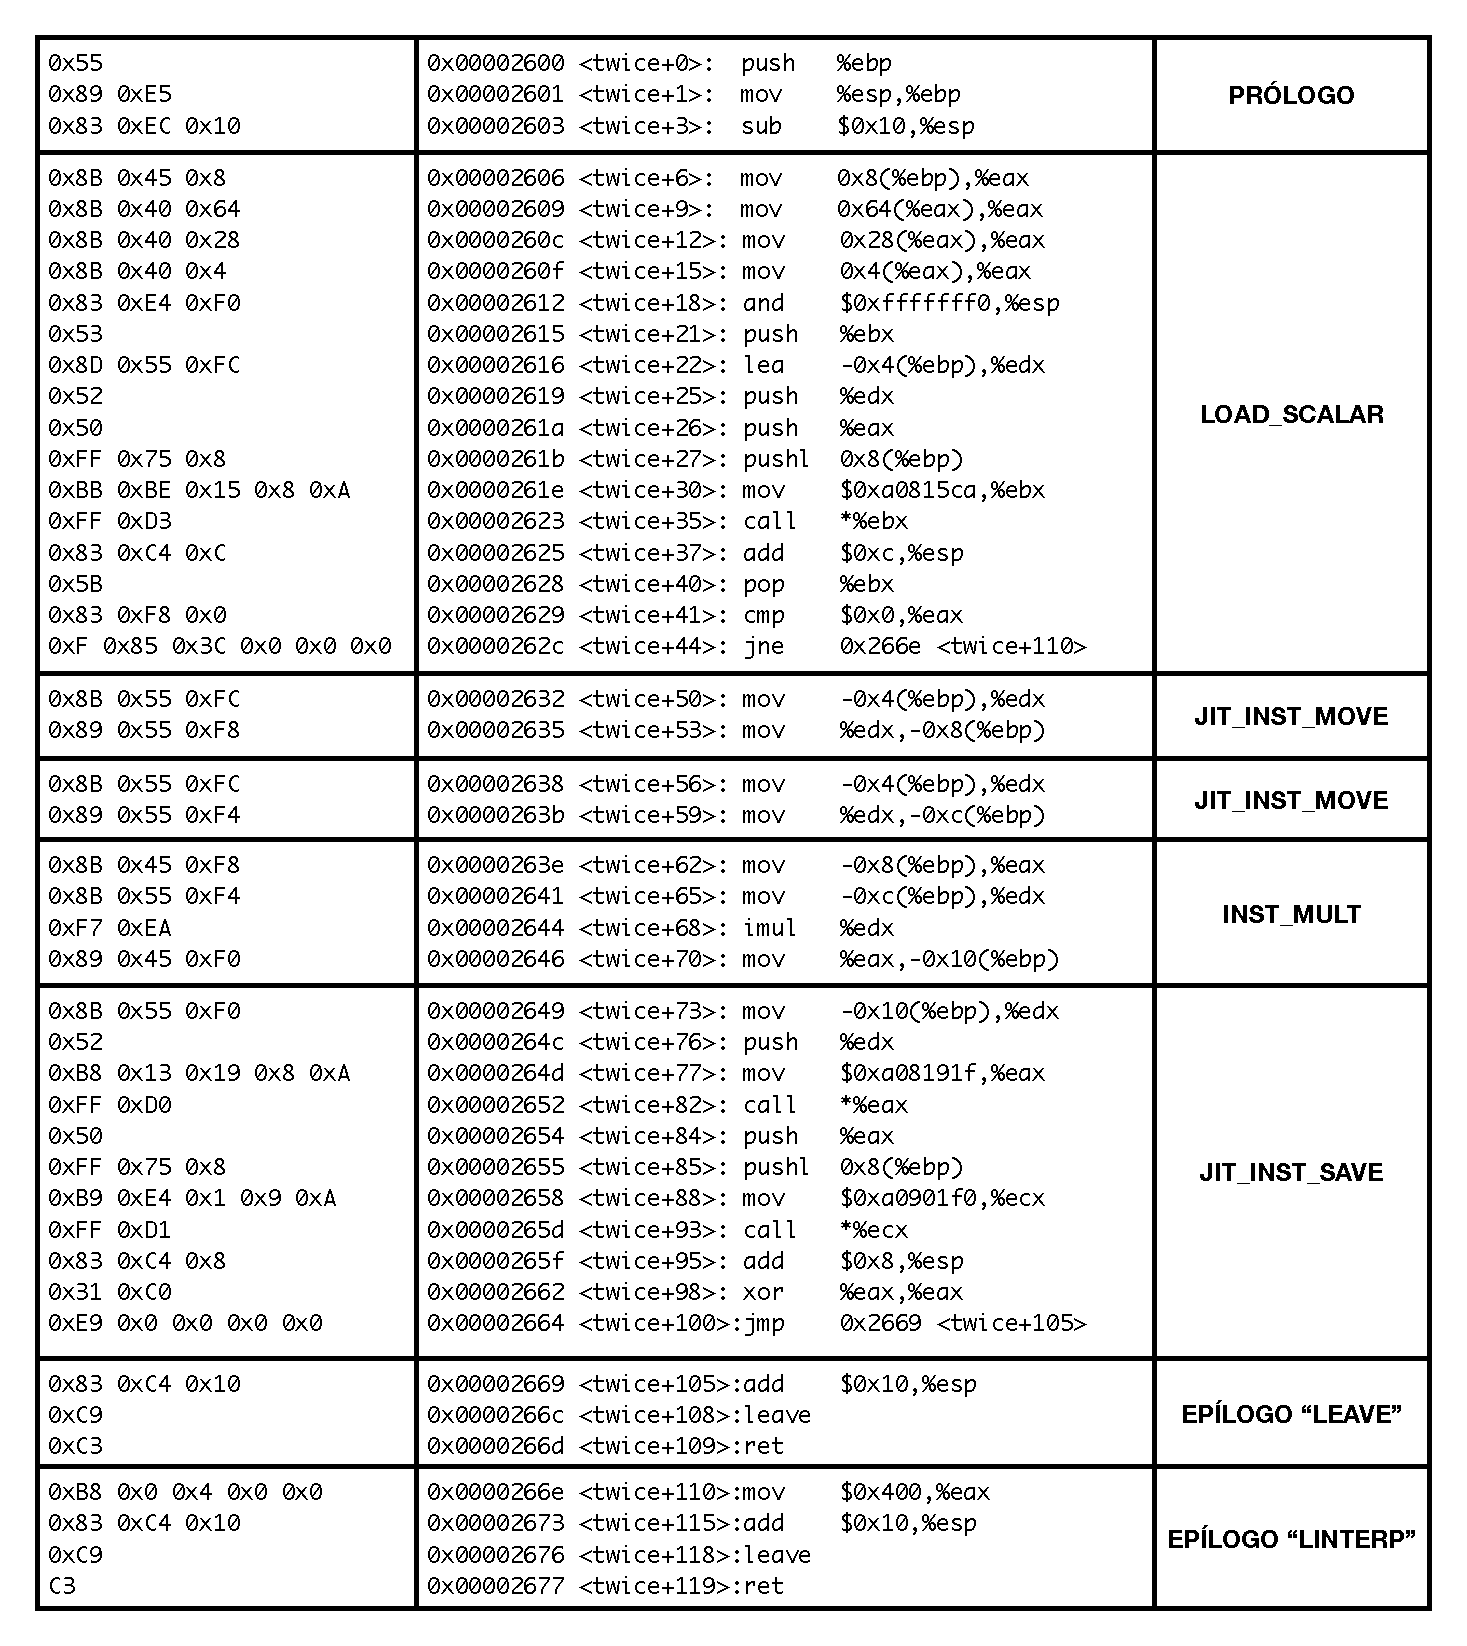
\includegraphics[scale=0.68]{figs/codelongo}
\end{table}

Apesar do procedimento codificado ser bastante simples, é possível
reutilizar código para outras instruções.
 A parte do código que acessa
variáveis locais é reaproveitada pelo código que acessa objetos
literais, com pequenas modificações. A movimentação entre
registradores é utilizada na grande maioria das instruções aceitas, e
com pequenas modificações no código da instrução de multiplicação
consegue-se realizar outras operações aritméticas.

% XXX Talvez colocar alguma coisa assim, melhor explicado.
%Devido a dinamicidade da linguagem \texttt{Tcl}, a coleta de
%tipos realizada em tempo de execução não conseguiu demonstrar
%utilidade na geração de código.
%acabou não demonstrado uso real na geração de código. Seria
%necessário uma forma eficiente para determinação de tipos, mas não
%foi encontrado.
